\documentclass[11pt,a4paper]{article}\usepackage[utf8]{inputenc}

\usepackage[T1]{fontenc}
\usepackage{tgpagella}
\usepackage[spanish]{babel}
\usepackage{geometry}
\usepackage{graphicx}
\usepackage{booktabs}
\usepackage{array}
\usepackage{xcolor}
\usepackage{titlesec}
\usepackage{fancyhdr}
\usepackage[parfill]{parskip}
\usepackage[expansion=false]{microtype}
\usepackage{hyperref}
\usepackage{setspace}
\usepackage{needspace}

\geometry{top=3.0cm,bottom=3.0cm,left=3.5cm,right=3.5cm}
\setlength{\parskip}{0.65em}
\setlength{\parindent}{0em}

\definecolor{azulai}{RGB}{30,80,140}
\definecolor{doradoai}{RGB}{140,90,0}
\definecolor{grisai}{RGB}{70,70,70}

\titleformat{\section}{\Large\bfseries\color{azulai}}{}{0em}{}[{\color{azulai}\titlerule[0.5pt]\nopagebreak[4]}]
\titlespacing*{\section}{0pt}{1.8em}{0.8em}
\titleformat{\subsection}{\large\bfseries\color{doradoai}}{}{0em}{}[{\nopagebreak[4]}]
\titlespacing*{\subsection}{0pt}{1.4em}{0.5em}
\titleformat{\subsubsection}{\normalsize\bfseries\color{grisai}}{}{0em}{}[{\nopagebreak[4]}]
\titlespacing*{\subsubsection}{0pt}{1.0em}{0.3em}

\pagestyle{fancy}\fancyhf{}
\rhead{\textcolor{grisai}{\small Amay — Arquitectura Interna}}
\lhead{\textcolor{grisai}{\small Carta Natal Completa}}
\cfoot{\textcolor{grisai}{\small\thepage}}
\renewcommand{\headrulewidth}{0.3pt}

\hypersetup{colorlinks=true,linkcolor=azulai,urlcolor=azulai}
\setstretch{1.45}
\tolerance=1500
\emergencystretch=4em

\begin{document}

% ── Portada ──────────────────────────────────────────────────────────────────
\begin{titlepage}
  \centering
  \vspace*{1.5cm}
  {\Huge\bfseries\color{azulai} Carta Natal Completa}\\[0.5cm]
  {\large\color{grisai} Arquitectura Interna}\\[0.3cm]
  {\small\itshape\color{grisai} Un método para sostener cuerpo, energía y vida con coherencia}\\[2cm]
  {\huge\color{doradoai} Amay}\\[1.5cm]
  {\Large 15/04/1588 \quad 11:15}\\[0.3cm]
  {\Large dfa}\\[0.3cm]
  {\normalsize Lat: 42.8473° \quad Lon: -2.6757° \quad UTC-00:15}\\[0.3cm]
  {\normalsize Ascendente: Leo 1°01' \quad
    MC: Aries 14°43'}\\[2.5cm]
  \vfill
  {\small Generado el 19/05/2026}
\end{titlepage}

\tableofcontents
\newpage

% ── Rueda ─────────────────────────────────────────────────────────────────────
\section{Carta Natal}
\begin{figure}[h!]
  \centering
  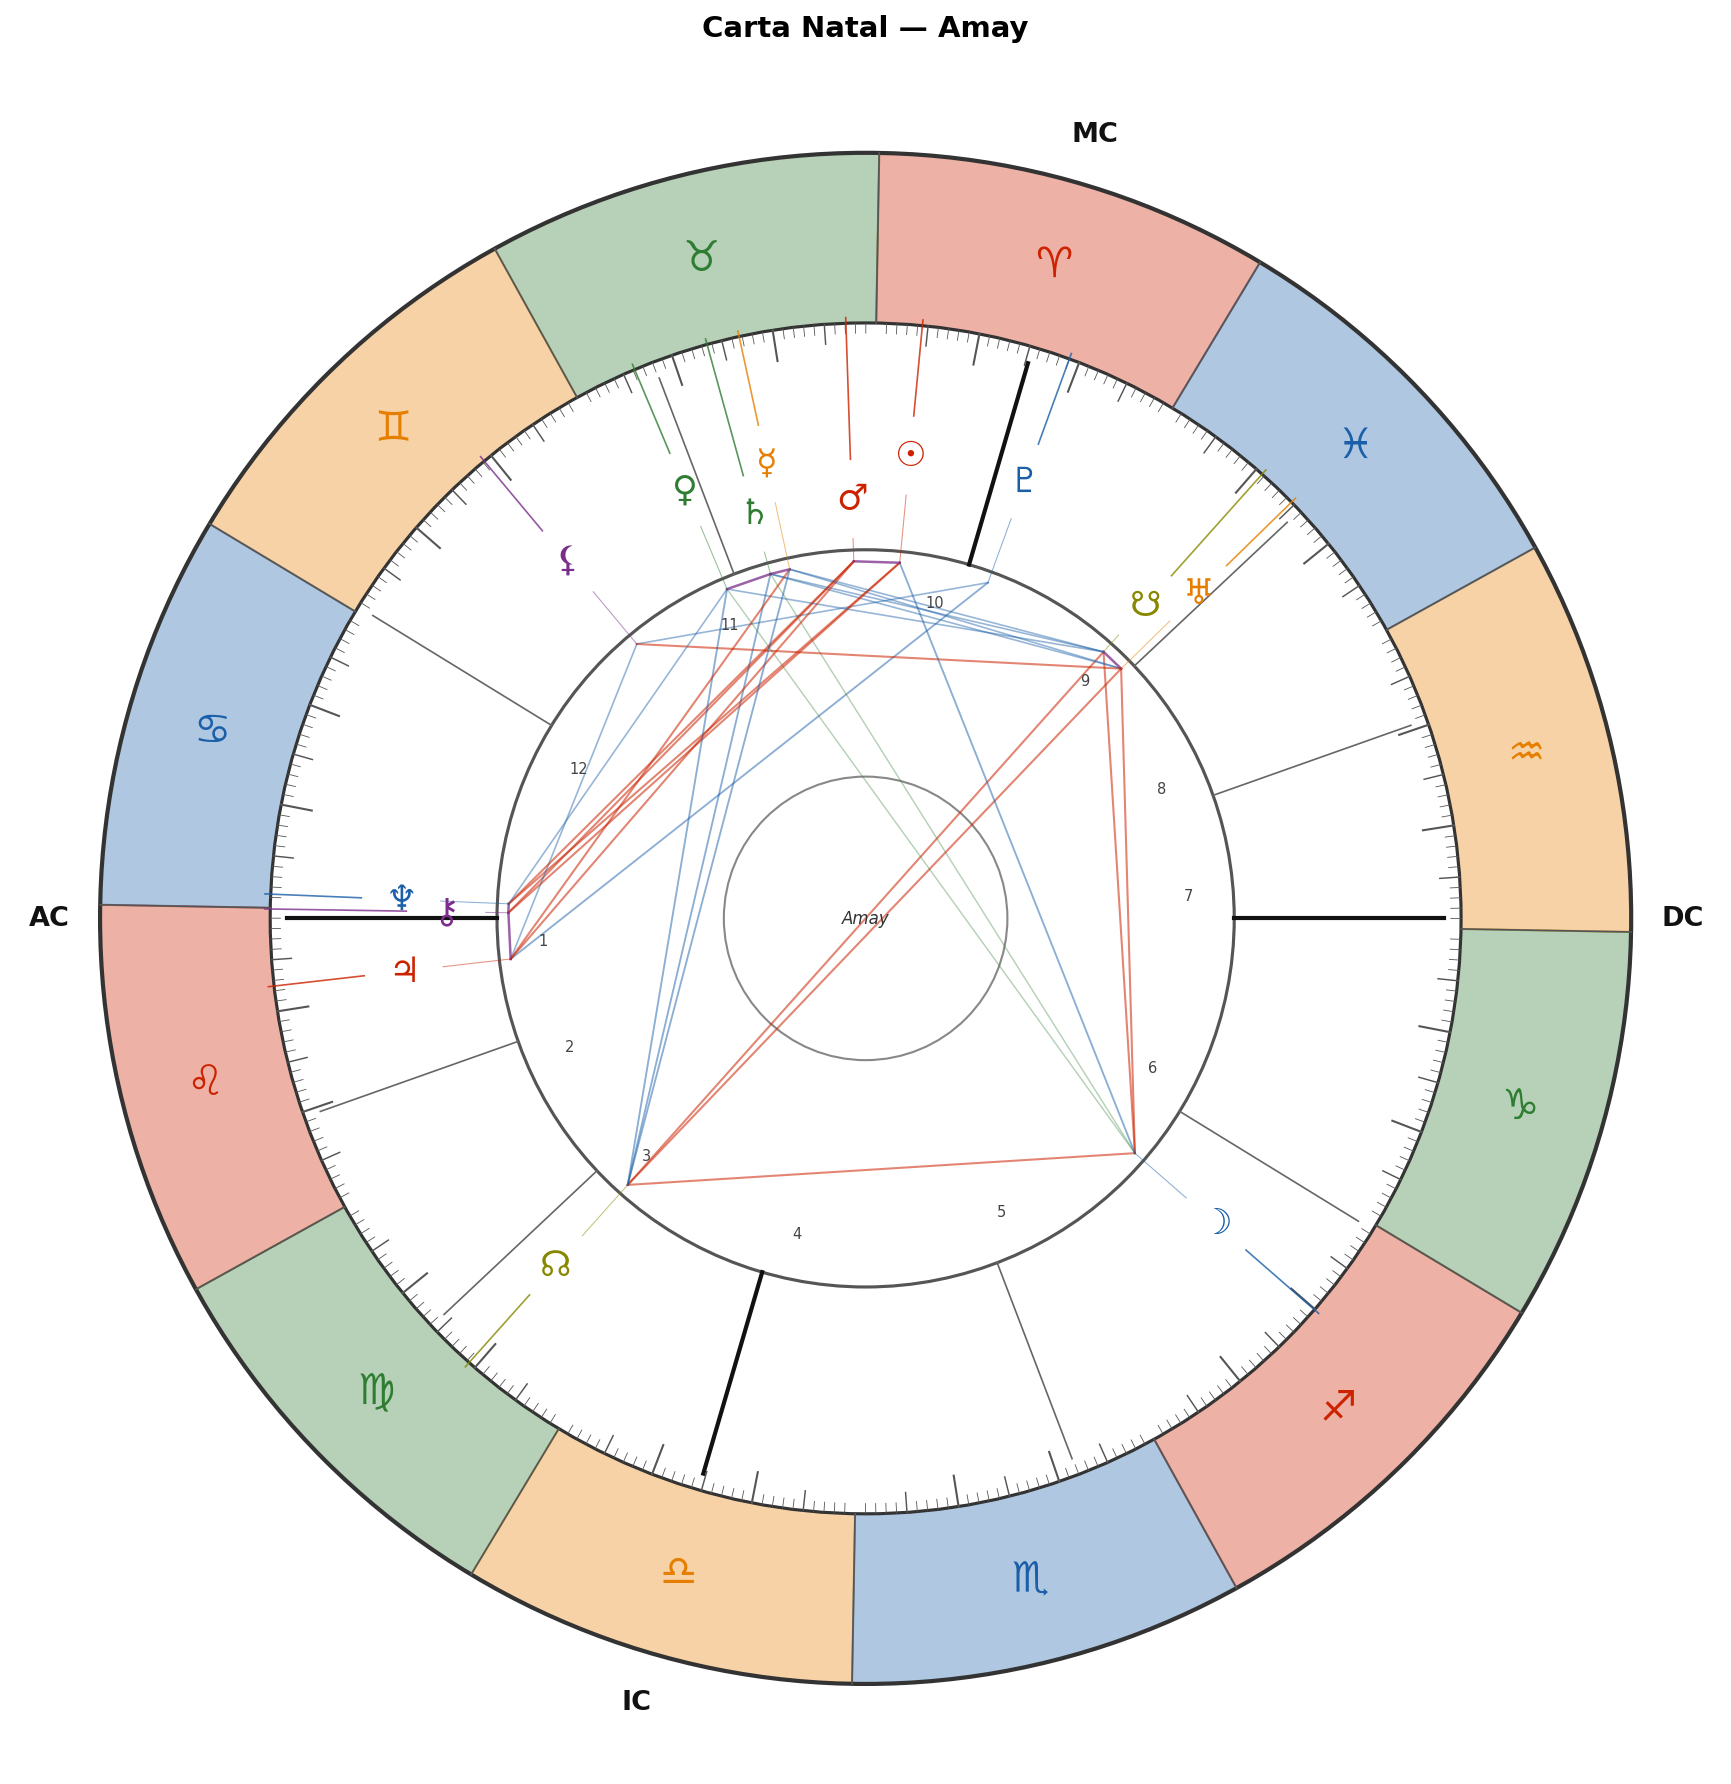
\includegraphics[width=0.90\textwidth]{Amay_AI_rueda.png}
  \caption{Carta natal de Amay — 15/04/1588 11:15 — dfa}
\end{figure}

\newpage

% ── Tabla de posiciones ───────────────────────────────────────────────────────
\section{Posiciones Planetarias}

\begin{center}
\begin{tabular}{llrrlll}
  \toprule
  \textbf{Planeta} & \textbf{Signo} & \textbf{Grado} & \textbf{Casa} &
  \textbf{Elemento} & \textbf{R} \\
  \midrule
  Sol & Aries & 25°33' & 10 & Fuego &  \\
  Luna & Sagitario & 19°56' & 5 & Fuego &  \\
  Mercurio & Tauro & 13°17' & 10 & Tierra &  \\
  Venus & Tauro & 23°51' & 11 & Tierra &  \\
  Marte & Tauro & 2°55' & 10 & Tierra &  \\
  Júpiter & Leo & 7°33' & 1 & Fuego &  \\
  Saturno & Tauro & 16°28' & 10 & Tierra &  \\
  Urano & Piscis & 15°22' & 9 & Agua &  \\
  Neptuno & Cáncer* & 28°41' & 12 & Agua &  \\
  Plutón & Aries & 11°00' & 9 & Fuego &  \\
  Quirón & Leo & 0°07' & 12 & Fuego &  \\
  Lilith & Géminis & 10°51' & 11 & Aire &  \\
  Nodo Norte & Virgo & 19°16' & 3 & Tierra &  \\
  Nodo Sur & Piscis & 19°16' & 9 & Agua &  \\
  \bottomrule
\end{tabular}
\end{center}

\vspace{0.5cm}
\begin{itemize}
  \item \textbf{Ascendente:} Leo 1°01'
  \item \textbf{Medio Cielo:} Aries 14°43'
  \item \textbf{Signos interceptados} (marcados con * en la tabla):
  \begin{itemize}
  \item Cáncer (casa 12) -- Capricornio (casa 6)
  \end{itemize}
\end{itemize}

\newpage

% ── Interpretación ────────────────────────────────────────────────────────────
\section{Interpretación — Arquitectura Interna}

\begin{center}
{\small\itshape
No se trata de definirte. Se trata de observar cómo se organiza tu energía,\
dónde puedes perder equilibrio y qué apoyos te ayudan a sostenerte.
}
\end{center}

\vspace{0.5cm}

\subsection{1. Visión General}

Tu carta muestra la siguiente distribución de elementos: Fuego 9, Tierra 5.5, Aire 0, Agua 2. Fuego (vitalidad, iniciativa, necesidad de sentido y movimiento hacia la acción) y Tierra (arraigo en lo concreto, estructura material, ritmo sostenido y contacto con el cuerpo): ahí está el peso de tu carta. Es el registro desde el que tu energía se activa con más fluidez y sin esfuerzo consciente. Agua (profundidad emocional, capacidad de resonancia, sensibilidad abierta) y Aire (desapego, análisis, pensamiento relacional y capacidad de perspectiva) está poco representado en tu carta. Ese territorio puede pedirte un esfuerzo consciente, especialmente cuando la presión sube. La mayoría de tus planetas están en signos fijos: hay capacidad de persistencia, estabilidad y continuidad. Cuando algo tiene sentido para ti, puedes sostenerlo durante mucho tiempo incluso en condiciones difíciles. La dificultad aparece cuando hace falta cambiar de dirección y una parte de ti sigue intentando mantener lo conocido. Tu Medio Cielo en Aries: La iniciativa directa, el liderazgo propio y la capacidad de iniciar. Tu presencia profesional tiende a percibirse como activa e independiente.

\vspace{0.8cm}
\Needspace{5\baselineskip}

\subsection{2. Ejes Principales}

\subsubsection*{Sol en Aries — Casa 10}
Tu Sol en Aries necesita pasar a la acción antes de que todo esté listo. Tu energía se enciende sola ante un reto o un proyecto nuevo, y puede apagarse si no hay movimiento. Sin algo en marcha o una dirección clara, puedes sentir irritación, vacío o necesidad de activar algo rápidamente. El riesgo no es la falta de energía sino arrancar sin base suficiente y quedarte vacío después del impulso. En Casa 10, tu identidad está ligada al espacio público, la vocación y el reconocimiento social. Tienes una necesidad real de construir algo visible que tenga coherencia contigo. Tu desarrollo profesional no es solo carrera: tiene un peso directo en tu forma de estar en el mundo.

\subsubsection*{Luna en Sagitario — Casa 5}
Tu Luna en Sagitario necesita movimiento, perspectiva y sentido. Cuando algo te afecta, te ayuda entender para qué sirve, hacia dónde te lleva o qué puedes hacer con ello. Si no encuentras una salida, el estado emocional puede convertirse en inquietud, impaciencia o necesidad de cambiar de escenario. El movimiento, el cambio de perspectiva y la sensación de amplitud te ayudan a recuperar estabilidad. En Casa 5, tu seguridad emocional se activa a través de la expresión creativa, el juego y el amor. Necesitas que tu vida emocional tenga un componente de disfrute y de expresión auténtica.

\subsubsection*{Ascendente Leo}
Tu Ascendente en Leo hace que te muestres al mundo con calidez, presencia y una orientación natural a ocupar el espacio con seguridad. Entras al entorno con una energía que otros notan. La necesidad de expresarte y ocupar espacio suele percibirse desde el primer contacto. Su regente es el Sol, en Aries y Casa 10. El Ascendente toma el tono de Aries: directa, rápida y orientada a la acción. Esa energía opera principalmente desde la vocación, la responsabilidad y el espacio público.

\subsubsection*{Grados finales de signo}
Los grados finales de signo suelen hablar de zonas de la carta donde hay mucha experiencia acumulada y sensación de       cierre de etapa. La energía no se vive de forma ligera o automática: suele haber más intensidad, más consciencia y la sensación de que una forma antigua de funcionar ya no termina de encajar igual.

No significa algo negativo ni indica un destino fijo. Simplemente muestra lugares donde la vida suele pedir más presencia, más maduración y una manera distinta de responder.

También aparecen posiciones en grados previos al anarético. No suelen sentirse tan extremos como el grado 29, pero sí muestran zonas donde ya existe bastante maduración y donde empiezan a aparecer señales de cambio o agotamiento de una forma antigua de funcionar.

Neptuno en Cáncer 28°41', Casa 12 aparece en grado previo al anarético. Eres especialmente sensible al ambiente, a las emociones de otras personas y a todo lo que ocurre alrededor. Cuando no hay suficiente descanso, silencio o límites claros, puedes terminar absorbiendo demasiado y perder claridad sobre lo que realmente necesitas. No todo lo que sientes es necesariamente tuyo. Aprender a diferenciarlo cambia mucho tu equilibrio interno.

Cuando varios puntos de la carta están al final de signo, la vida puede sentirse más intensa o vivirse con menos sensación de margen interno. A veces aparece urgencia, cansancio de ciertas dinámicas o sensación de estar cerca de cambios importantes incluso aunque externamente todo siga igual.

No significa que la vida vaya a ser más difícil. Significa que esas zonas necesitan más consciencia, más pausa y una forma más presente de responder, en lugar de seguir funcionando únicamente desde hábitos automáticos.


\subsubsection*{Signos interceptados}
Los signos Cáncer (Casa 12) con Neptuno y Capricornio (Casa 6) aparecen interceptados: su expresión puede sentirse menos inmediata o menos natural al principio. Esto influye especialmente en Neptuno, que pueden necesitar más tiempo, experiencia o situaciones concretas para sentirse plenamente desarrollados. Muchas veces estas posiciones no se muestran rápido desde fuera, pero ganan fuerza y claridad con los años.

\vspace{0.8cm}
\Needspace{5\baselineskip}

\subsection{3. Organización de la Energía}

Tu Mercurio en Tauro necesita tiempo para procesar. No suele llegar a conclusiones por impulso, pero cuando algo se asienta, resulta difícil moverlo. Piensas mejor cuando hay calma, continuidad y contacto con lo concreto. En Casa 10, la forma de pensar y comunicarte influye directamente en tu espacio profesional o público. Tus ideas, palabras o capacidad de organización pueden tener impacto visible en tu trayectoria. Tu Venus en Tauro necesita estabilidad, presencia y gestos concretos. El afecto se sostiene mejor cuando hay continuidad, confianza y contacto real. El riesgo aparece cuando la necesidad de seguridad dificulta cambiar una dinámica que ya no nutre. En Casa 11, el afecto se desarrolla mejor cuando hay amistad, intercambio y proyectos compartidos. Necesitas sentir que la relación también funciona como espacio de libertad y conexión humana. Tu Marte en Tauro actúa despacio, pero con mucha persistencia. No se activa por cualquier cosa, pero cuando toma dirección puede sostenerla durante mucho tiempo. El riesgo aparece cuando la resistencia al cambio te mantiene en una posición más de lo necesario. En Casa 10, la acción se orienta fuertemente hacia objetivos, reconocimiento y construcción profesional. Hay capacidad para sostener esfuerzo cuando existe una meta clara.

\vspace{0.8cm}
\Needspace{5\baselineskip}

\subsection{4. Estructura y Tensión}

\subsubsection*{Concentración de energía}

Hay una concentración notable en Casa 10: Sol, Mercurio, Marte y Saturno. Cuando varios planetas ocupan la misma casa, esa área absorbe buena parte de la actividad vital. En esta carta, el foco de la vocación, la responsabilidad y el espacio público funciona como núcleo central: ahí se acumula la presión, la demanda es mayor y también hay más recursos disponibles para operar. No es necesariamente un conflicto, pero sí un punto de alta intensidad sostenida.

También hay una concentración significativa en Casa 9: Urano, Plutón y Nodo Sur. En este caso, el foco se desplaza hacia el aprendizaje, la expansión y la necesidad de ampliar horizontes. Es un ámbito donde la exigencia aumenta, donde se concentra parte de la presión y donde también existe capacidad real de sostener procesos importantes. Tampoco es en sí un problema, pero sí un área de intensidad mantenida.



Los aspectos aparecen organizados en dos niveles. Los aspectos exactos (orbe igual o menor a 1°) suelen sentirse de forma más inmediata y constante en la vida cotidiana. Los aspectos estructurales tienen un orbe más amplio, pero siguen describiendo dinámicas importantes que se repiten a lo largo de la vida.



\vspace{0.8cm}
\Needspace{5\baselineskip}
\subsubsection*{Aspectos exactos}
No aparecen aspectos exactos especialmente fuertes dentro del orbe definido para esta lectura. Eso no significa ausencia de tensión o profundidad, sino que gran parte de las dinámicas importantes de la carta se construyen de forma más amplia y progresiva. En este caso, cobran más importancia los aspectos estructurales y la combinación general de posiciones.

\vspace{0.8cm}
\Needspace{5\baselineskip}
\subsubsection*{Aspectos estructurales}
\Needspace{3\baselineskip}
\subsubsection*{Sol (Casa 10) conjunción Marte (Casa 10) --- orbe 7.37\textdegree}
La conjunción Sol-Marte une identidad y acción. Cuando tienes una dirección clara, puedes actuar con rapidez, iniciativa y mucha fuerza disponible. Cuando no hay salida concreta, esa fuerza puede convertirse en impaciencia, tensión o necesidad de intervenir. Este aspecto pide objetivos claros para que la acción no se transforme en desgaste.



\vspace{0.8cm}
\Needspace{5\baselineskip}

\subsection{5. Sostén y Equilibrio}

Tu Quirón en Leo, Casa 12, señala una zona sensible relacionada con la expresión personal, el reconocimiento y la posibilidad de mostrarte tal como eres. Puede que aprendieras a contenerte para no destacar demasiado o para evitar exponerte. Esto suele notarse especialmente en la vida privada, la necesidad de retiro y lo que cuesta mostrar. No significa que tengas límites en ese terreno, pero sí que probablemente necesites más tiempo, cuidado o consciencia para sentir estabilidad ahí.

\vspace{0.3cm}
Tu Nodo Sur en Piscis, Casa 9, muestra una tendencia a moverte desde la falta de límites claros, la adaptación excesiva o la tendencia a perderte en el entorno, especialmente en el aprendizaje, las creencias y la necesidad de ampliar horizontes. Suele ser una forma de funcionar conocida o automática para ti. Tu Nodo Norte en Virgo, Casa 3, señala la necesidad de desarrollar orden, presencia en lo cotidiano y capacidad de concretar, especialmente en la comunicación y el entorno cercano. No se trata de rechazar lo anterior, sino de ampliar tu forma habitual de responder.

\vspace{0.3cm}
En tu carta hay poca presencia de Aire. Cuando aparece saturación, bloqueo o sensación de desorganización interna, suele ayudarte volver a espacios relacionados con la perspectiva, el espacio mental y las conversaciones que ordenan. Eso puede darte más estabilidad y ayudarte a recuperar claridad.

\vspace{0.8cm}
\Needspace{5\baselineskip}

\subsection{6. Orientación}

\subsubsection*{Qué observar}
Tu Ascendente en Leo describe la forma en que otras personas suelen percibirte al principio. Eso no siempre coincide con cómo vives las cosas internamente o con las tensiones más importantes de tu carta. Cuando hay demasiada distancia entre lo que muestras y lo que realmente te ocurre, aparece desgaste.

\subsubsection*{Qué puede desestabilizar}
Hay ciertas tensiones en tu carta que pueden activarse con bastante fuerza: Nodo Norte-Nodo Sur, Luna-Nodo Norte, Luna-Nodo Sur. Cuando varias coinciden al mismo tiempo, puede aparecer sensación de saturación, reacción excesiva o dificultad para mantener claridad.

\subsubsection*{Qué estructura y sostiene}
Tu Sol en Aries, Casa 10, muestra un terreno importante de estabilidad para ti. Cuando tu forma de actuar está alineada con lo que realmente valoras, suele aparecer más claridad y menos dispersión.

\subsubsection*{Orientación práctica}
Una orientación práctica: en tu carta hay poco Aire. Cuando las emociones o las tensiones aumentan, puede costarte tomar distancia y ordenar lo que te ocurre. Escribir, hablar con alguien de confianza o darte tiempo antes de reaccionar puede ayudarte mucho más de lo que parece.

\vspace{1cm}
\begin{center}
{\small\itshape\color{grisai}
La astrología se usa aquí como lenguaje simbólico de observación, no como una definición de quién eres.\\
Esta interpretación es tu mapa de posibilidades, no tu destino fijo.
}
\end{center}

\end{document}
